\documentclass[tikz,border=2pt]{standalone}
\usepackage{tikz}
\usetikzlibrary{arrows.meta,positioning,calc,decorations.pathmorphing}
\begin{document}
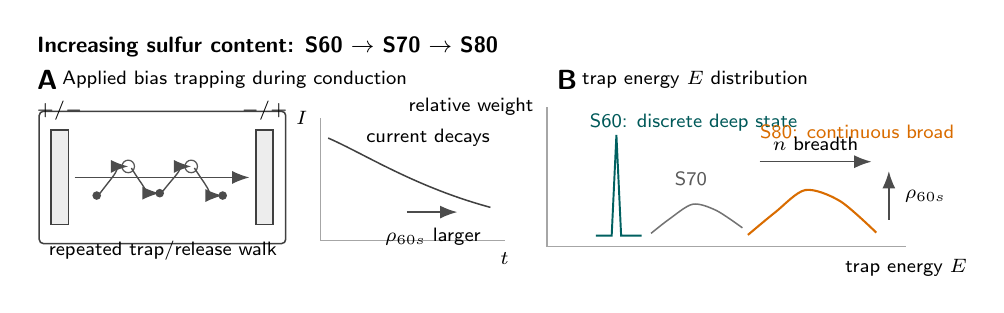
\begin{tikzpicture}[
  font=\sffamily\scriptsize,
  >=Latex,
  line/.style={draw=black!75,line width=0.55pt},
  soft/.style={draw=black!35,line width=0.45pt},
  ion/.style={circle,fill=black!70,inner sep=1.1pt},
  trap/.style={circle,draw=black!65,fill=white,line width=0.45pt,inner sep=1.6pt},
  deep/.style={circle,draw=teal!70!black,fill=teal!13,line width=0.55pt,inner sep=1.8pt},
  broad/.style={circle,draw=orange!80!black,fill=orange!15,line width=0.45pt,inner sep=1.4pt},
  cue/.style={draw=black!70,line width=0.5pt,-{Latex[length=2.2mm]}}
]

% Header
\node[font=\sffamily\footnotesize\bfseries,anchor=west] at (-0.1,3.24)
  {Increasing sulfur content: S60 \(\rightarrow\) S70 \(\rightarrow\) S80};

% Panel A
\node[font=\sffamily\bfseries,anchor=west] at (-0.1,2.82) {A};
\node[anchor=west] at (0.22,2.82) {Applied bias trapping during conduction};

\draw[line,rounded corners=1.5pt] (0.05,0.74) rectangle (3.18,2.42);
\draw[line,fill=black!7] (0.20,0.98) rectangle (0.42,2.18);
\draw[line,fill=black!7] (2.80,0.98) rectangle (3.02,2.18);
\node[anchor=south] at (0.31,2.18) {\(+/-\)};
\node[anchor=south] at (2.91,2.18) {\(-/+\)};
\draw[cue] (0.50,1.58) -- (2.72,1.58);
\node[ion] at (0.78,1.35) {};
\node[trap] at (1.18,1.72) {};
\node[ion] at (1.58,1.38) {};
\node[trap] at (1.98,1.72) {};
\node[ion] at (2.38,1.35) {};
\draw[cue] (0.80,1.35) .. controls (1.00,1.62) and (1.12,1.72) .. (1.18,1.72);
\draw[cue] (1.22,1.70) .. controls (1.36,1.47) and (1.46,1.38) .. (1.58,1.38);
\draw[cue] (1.60,1.38) .. controls (1.80,1.64) and (1.92,1.72) .. (1.98,1.72);
\draw[cue] (2.02,1.70) .. controls (2.16,1.48) and (2.28,1.35) .. (2.38,1.35);
\node[anchor=north] at (1.62,0.90) {repeated trap/release walk};

\begin{scope}[shift={(3.62,0.78)}]
  \draw[soft] (0,0) -- (2.34,0);
  \draw[soft] (0,0) -- (0,1.56);
  \node[anchor=north] at (2.34,-0.03) {\(t\)};
  \node[anchor=east] at (-0.04,1.56) {\(I\)};
  \draw[line] (0.10,1.30) .. controls (0.56,1.10) and (1.20,0.68) .. (2.16,0.42);
  \node[anchor=west] at (0.46,1.30) {current decays};
  \draw[cue] (1.10,0.36) -- (1.74,0.36);
  \node[anchor=north] at (1.43,0.28) {\(\rho_{60s}\) larger};
\end{scope}

% Panel B
\node[font=\sffamily\bfseries,anchor=west] at (6.50,2.82) {B};
\node[anchor=west] at (6.82,2.82) {trap energy \(E\) distribution};

\begin{scope}[shift={(6.50,0.70)}]
  \draw[soft] (0,0) -- (4.56,0);
  \draw[soft] (0,0) -- (0,1.78);
  \node[anchor=north] at (4.56,-0.03) {trap energy \(E\)};
  \node[anchor=east] at (-0.05,1.78) {relative weight};

  \draw[teal!75!black,line width=0.7pt]
    (0.62,0.14) -- (0.82,0.14) -- (0.88,1.42) -- (0.94,0.14) -- (1.20,0.14);
  \node[teal!70!black,anchor=west] at (0.42,1.58) {S60: discrete deep state};

  \draw[black!55,line width=0.55pt]
    plot[smooth] coordinates {(1.32,0.17) (1.55,0.35) (1.85,0.54) (2.15,0.46) (2.48,0.24)};
  \node[black!65,anchor=west] at (1.50,0.86) {S70};

  \draw[orange!85!black,line width=0.75pt]
    plot[smooth] coordinates {(2.55,0.15) (2.90,0.44) (3.28,0.72) (3.72,0.58) (4.18,0.18)};
  \node[orange!85!black,anchor=west] at (2.58,1.46) {S80: continuous broad};

  \draw[cue] (2.70,1.08) -- (4.12,1.08);
  \node[anchor=south] at (3.41,1.10) {\(n\) breadth};
  \draw[cue] (4.34,0.34) -- (4.34,0.96);
  \node[anchor=west] at (4.42,0.64) {\(\rho_{60s}\)};
\end{scope}

\end{tikzpicture}
\end{document}
